%%% Exemplo de utilização da classe ITA
%%%
%%%   por        Fábio Fagundes Silveira   -  ffs [at] ita [dot] br
%%%              Benedito C. O. Maciel     -  bcmaciel [at] ita [dot] br
%%%              Giovani Volnei Meinertz   -  giovani [at] ita [dot] br
%%%    	         Hudson Alberto Bode       -  bode [at] ita [dot]br
%%%    	         P. I. Braga de Queiroz    -  pi [at] ita [dot] br
%%%    	         Jorge A. B. Gripp         -  gripp [at] ita [dot] br
%%%    	         Juliano Monte-Mor         -  jamontemor [at] yahoo [dot] com [dot] br
%%%    	         Tarcisio A. B. Gripp      -  tarcisio.gripp [at] gmail [dot] com
%%%
%%%   Versão para overleaf:
%%%   por        Alejandro A. Rios Cruz    - aarc.88@gmail.com
%%%              Saulo Gómez               - sagomezs@unal.edu.co
%%%              Ocimar Santos             - ocimar.acad@gmail.com
%%%
%%%   Template disponibilizado em:
%%%              Overleaf: https://pt.overleaf.com/latex/templates/thesis-template-aeronautics-institute-of-technology-ita/yhfrqqydpygk
%%%
%%%   Contribuia você também!
%%%              GitHub:   https://github.com/AlejandroRios/Template_Thesis_ITA
%%%
%%%  IMPORTANTE: O texto contido neste exemplo nao significa absolutamente nada.  :-)
%%%              O intuito aqui eh demonstrar os comandos criados na classe e suas
%%%              respectivas utilizacoes.
%%%
%%%  Tese.tex  2016-08-25
%%%  $HeadURL: http://www.apgita.org.br/apgita/teses-e-latex.php $
%%%
%%% ITALUS
%%% Instituto Tecnológico de Aeronáutica --- ITA, Sao Jose dos Campos, Brasil
%%%                   http://groups.yahoo.com/group/italus/
%%% Discussion list: italus {at} yahoogroups.com
%%%
%++++++++++++++++++++++++++++++++++++++++++++++++++++++++++++++++++++++++++++++
% Para alterar o TIPO DE DOCUMENTO, preencher a linha abaixo \documentclass[?]{?}
%   \documentclass[tg]{ita}			= Trabalho de Graduacao
%   \documentclass[tgfem]{ita}	= Para Engenheiras
%   								msc     		= Dissertacao de Mestrado
%   								mscfem   		= Para Mestras
%   								dsc      		= Tese de Doutorado
%   								dscfem   		= Para Doutoras
%   								quali    		= Exame de Qualificacao
%   								qualifem 		= Exame de Qualificacao para Doutoras
% Para 'Draft Version'/'Versao Preliminar' com data no rodape, adicionar 'dv':
%   \documentclass[dsc, dv]{ita}
% Para trabalhos em Inglês, adicionar 'eng':
%   \documentclass[dsc, eng]{ita}
%		\documentclass[dsc, eng, dv]{ita}
%++++++++++++++++++++++++++++++++++++++++++++++++++++++++++++++++++++++++++++++
\documentclass[tg, eng]{ita}    % ITA.cls based on standard book.cls
% Quando alterar a classe, por exemplo de [msc] para [msc, eng]) rode mais uma vez o botão BUILD OUTPUT caso haja erro
\usepackage[utf8]{inputenc}
\usepackage{ae}
\usepackage{graphicx}
\usepackage{epsfig}
\usepackage{amsmath}
\usepackage{amssymb}
\usepackage{subcaption}
\usepackage{multirow}
\usepackage{float}
\usepackage{amsthm}
\usepackage{url}         % formats URL addresses properly
\usepackage{appendix}    % allows appendix section to be included
\usepackage{lscape}      % allows a page to be rendered in landscape mode
\usepackage{multicol}    % allows text in multi columns
\usepackage{cancel}      % needed to show canceled terms in equations
\usepackage{lettrine}
\usepackage{float}
\usepackage{placeins}
\usepackage{tikz}
\usetikzlibrary{shapes.geometric, arrows, positioning}

\tikzstyle{startstop} = [rectangle, rounded corners, 
minimum width=3cm, 
minimum height=1cm,
text centered, 
draw=black, 
fill=red!30]

\tikzstyle{io} = [trapezium, 
trapezium stretches=true, % A later addition
trapezium left angle=70, 
trapezium right angle=110, 
minimum width=3cm, 
minimum height=1cm, text centered, 
draw=black, fill=blue!30]

\tikzstyle{process} = [rectangle, 
minimum width=3cm, 
minimum height=1cm, 
text centered, 
text width=3cm, 
draw=black, 
fill=lightgray!30]

\tikzstyle{decision} = [diamond, 
% minimum width=1cm, 
% minimum height=1cm, 
text centered, 
draw=black, 
fill=green!30]
\tikzstyle{arrow} = [thick,->,>=stealth]


%HHHHHHHHHHHHHHHHHHHHHHHHHHHHHHHHHHHHHHHHHHHHHHHHHHHHHHHHHHHHHHHHHHHHHHHHHHHHHHHHHHHHHHHHHHHHHHHHHHHHHHHHHHHH
%\usepackage{subfigure}
%\usepackage{subfigmat}
%PACOTEFIGURAS_SE _ERRADO_ESXCLUIR_ACIMA
\usepackage{booktabs}
%PACOTETABELAS_SE _ERRADO_ESXCLUIR_ACIMA
%HHHHHHHHHHHHHHHHHHHHHHHHHHHHHHHHHHHHHHHHHHHHHHHHHHHHHHHHHHHHHHHHHHHHHHHHHHHHHHHHHHHHHHHHHHHHHHHHHHHHHHHHHHHH

\newcommand{\x}{\mathbf{x}}
\newcommand{\pos}{\mathbf{r}}
\newcommand{\vel}{\mathbf{v}}
\newcommand{\acc}{\mathbf{a}}
\newcommand{\uc}{\mathbf{u}}
\newcommand{\R}{\mathbb{R}}
\newcommand{\N}{\mathbb{N}}


%++++++++++++++++++++++++++++++++++++++++++++++++++++++++++++++++++++++++++++++
% Espaçamento padrão de todo o documento
%++++++++++++++++++++++++++++++++++++++++++++++++++++++++++++++++++++++++++++++
\onehalfspacing

%singlespacing Para um espaçamento simples
%onehalfspacing Para um espaçamento de 1,5
%doublespacing Para um espaçamento duplo

%++++++++++++++++++++++++++++++++++++++++++++++++++++++++++++++++++++++++++++++
% Identificacoes (se o trabalho for em inglês, insira os dados em inglês)
% Para entradas abreviadas de Professora (Profa.) em português escreva: Prof$^\textnormal{a}$.
%++++++++++++++++++++++++++++++++++++++++++++++++++++++++++++++++++++++++++++++
\course{Aerospace Engineering}  % Programa de PG ou Curso de Graduação
%\area{Aircraft Design} % Área de concentração na PG (Não utilizado no caso de TG)

% Autor do trabalho: Nome Sobrenome
\authorgender{masc}                     %sexo: masc ou fem
\author{Pedro Kuntz}{Puglia}
\itaauthoraddress{Rua H8C, Ap. 303}{12.228- 462}{São José dos Campos- SP}

% Titulo da Tese/Dissertação
\title{Primer Vector Analysis of Optimal Impulsive Orbital Maneuvers Under Conservative and Non-Conservative Models}
% Orientador
\advisorgender{masc}                    % masc ou fem
\advisor{Prof.~Dr.}{Willer Gomes dos Santos}{ITA}

% Coorientador (Caso não haja coorientador, colocar ambas as variáveis \coadvisorgender e \coadvisor comentadas, com um % na frente)
\coadvisorgender{masc}									% masc ou fem
\coadvisor{Prof.}{Emilien Flayac}{ISAE-SUPAERO}

% Pró-reitor da Pós-graduação
% \bossgender{masc}												% masc ou fem
% \boss{Prof.~Dr.}{John von Neumann}

%Coordenador do curso no caso de TG
\bosscoursegender{fem}									% masc ou fem
\bosscourse{Profa.~Dra.}{Cristiane Martins}

% Palavras-Chaves informadas pela Biblioteca -> utilizada na CIP
\kwcip{Optimization}
\kwcip{Control}
\kwcip{Orbital Mechanics}

% membros da banca examinadora

% \examiner{Prof. Dr.}{Alan Turing}{Presidente}{ITA}
% \examiner{Prof. Dr.}{Linus Torwald}{}{UXXX}
% \examiner{Prof. Dr.}{Richard Stallman}{}{UYYY}
% \examiner{Prof. Dr.}{Donald Duck}{}{DYSNEY}
% \examiner{Prof. Dr.}{Mickey Mouse}{}{DISNEY}

% Data da defesa (mês em maiúsculo, se trabalho em inglês, e minúsculo se trabalho em português)
\date{??}{junho}{2025}

% Número CDU - (somente para TG)
\cdu{???.??}

% Glossario
\makeglossary
\frontmatter

\begin{document}
% Folha de Rosto e Capa para o caso do TG
\maketitle

% Dedicatoria: Nao esqueca essa secao  ... :-)
\begin{itadedication}
Aos amigos da Graduação e Pós-Graduação do ITA por motivarem tanto a criação deste template pelo Fábio Fagundes Silveira quanto por motivarem a mim e outras pessoas a atualizarem e aprimorarem este excelente trabalho.
\end{itadedication}

% Agradecimentos
\begin{itathanks}
Agradeço ao professor Leonardo Gouvêa por, certo dia falando sobre qualquer coisa, levantar a possibilidade deste trabalho, e por auxiliar no que é necessário auxílio e dar liberdade no que é necessário liberdade.

Agradeço também ao João Vitor Baldo e Arthur Zoppi, que acompanharam todas as minhas impressões 3D no Laboratório Aberto do CCM-ITA, sempre dando dicas e sugestões que iam além do esperado deles. Obrigado por transformar impressões problemáticas e fracassadas em momentos de descontração e aprendizado sobre mundo real.

Agradeço por fim a toda a equipe do Laboratório Feng, que foi recrutada por acaso no meio do caminho para minha iniciação científica. Agradeço ao Prof. Dr. Tiago Barbosa, que permitiu o uso do laboratório, e ao professor André Fernando de Castro, que certo dia por acaso resolveu (quase) todos os problemas experimentais do meu trabalho comigo. Agradeço especialmente aos técnicos Newton, que me auxiliou com toda a montagem mecânica do experimento, e Wilson, que me acompanhou pelas várias horas de montagem e calibração.

Por fim agradeço à minha família, que sempre me incentivou, e aos meus amigos de ITA e H8, que inúmeras vezes me ouviram falar detalhadamente sobre os problemas deste trabalho.
\end{itathanks}

% Epígrafe
\thispagestyle{empty}
\ifhyperref\pdfbookmark[0]{\nameepigraphe}{epigrafe}\fi
\begin{flushright}
\begin{spacing}{1}
\mbox{}\vfill
{\sffamily\itshape
``If I have seen farther than others,\\
it is because I stood on the shoulders of giants.''\\}
--- \textsc{Sir~Isaac Newton}

\end{spacing}
\end{flushright}

% Resumo
\begin{abstract}
\noindent
Este trabalho apresenta o processo de desenvolvimento e caracterização de um sistema de vetorização de empuxo com motor a gás frio. O motor tem como requisito empuxo de \(2\;\mathrm{N}\) e \(5\;\mathrm{bar}\) de pressão de câmara. O método de vetorização escolhido para teste foi o de \textit{jet vane}. O motor construído apresentou divergências pequenas com os requisitos, tendo um impulso específico de \(46,6\;\mathrm{s}\). Este motor foi montado em um mecanismo de controle da lâmina defletora e esta montagem foi acoplada a uma balança de três componentes para caracterização das forças e momentos gerados. Como resultado final, obtiveram-se as derivadas de controle de força lateral e momento. Por fim, apresentaram-se os problemas metodológicos encontrados e \textit{trade-offs} de engenharia identificados para o sistema.
\end{abstract}

% Abstract
\begin{englishabstract}
\noindent
This work presents the implementation of an orbital maneuver solver under two-body Keplerian dynamics and impulsive thrust model. The control task consists of finding the trajectory between two given states, in a fixed amount of time, minimizing fuel consumption. Optimal control formalism, in the form of the control Hamiltonian, is applied to the problem to uncover the consacrated primer vector theory, which can inform hyperparameter choice. A Julia interface to the recognized Ipopt solver is used to implement a relaxation method for the optimizer. A Lambert problem solver is used to supply a feasible initial guess to the solver. Finally, the results of direct optimization and primer vector theory are compared to the established Hohmann transfer analytical results to validate the implementation.
\end{englishabstract}

% Lista de figuras
\listoffigures %opcional

% Lista de tabelas
\listoftables %opcional

% Lista de abreviaturas
\printnoidxglossary[type=\acronymtype,
    title=\listofabbreviationsname,
    toctitle=\listofabbreviationsname,
    sort=standard,
    nonumberlist]
    
% Lista de simbolos
\printnoidxglossary[
    title=\listofsymbolsname,
    toctitle=\listofsymbolsname,
    sort=standard,
    nonumberlist]

% Sumario
\tableofcontents


\mainmatter

%todo
%resumo, abstract

% Os capitulos comecam aqui
\chapter{\textbf{Introduction}}
\section{Context}



% primeiro satelite manobravel


% discutir manobra interplanetária vs órbita terrestre

% GOCE

% daedalus

Space exploration relies on clever resource management, since satellites have a finite amount of resources (propellant and other consumables) to fulfill their mission. Up to this date, all space hardware is expendable, that is, when the consumables required for mission maintenance are finished, the mission ends, marking the end of the exploration of a very expensive engineered system. Thus the need for optimization arises in this domain.

Contrary to science fiction, where spaceships seem to be constantly propelled by their thrusters, real life satellites change their courses in discrete moments of maximum thrust application, surrounded by (usually long) coasting periods. This is due to the relatively high power delivered by traditional rocket engines, which can, in the matter of seconds or minutes, greatly alter a satelite's orbit. Certain more modern propulsion systems, such as electric rocket engines, are somewhat of an exception; this technicality will be discussed in further sections.

Orbital maneuvers are necessary in all stages of a satellite's lifecycle. In the beginning of a mission, the satellite is released by the launch vehicle in an orbit that is usually not the mission's orbit. Therefore, an \textit{injection maneuver} is necessary to bring the satellite into an operational orbit. This is usually the biggest maneuver a satellite must execute during its lifecycle, consuming a high fraction of its propellant storage. 

During a mission, the satellite must perform sporadic \textit{maintenance maneuvers}, which are small course correction maneuvers to mitigate external perturbations such as atmospheric drag, Earth's oblateness effects (if undesired), gravitational attraction of celestial bodies, and solar radiation pressure. Their frequency and magnitude vary depending on mission requirements, and in industrial applications, other mission requirements must be taken into account when planning maneuvers. The presence of sensitive sensors that must not be pointed at the Sun, solar panels that must always be illuminated, or events such as observation of a ground target are examples of sources of constraints on when maneuvers can be executed. Those are by far the most common type of maneuver, and a loose, non-exhaustive classification arises naturally.

The simplest type of maneuver is that of \textit{orbit raising}, which consists in bringing the satellite from a (often near-circular) orbit and increasing its semimajor-axis (and thus, its period) until a desired value. This maneuver is commonly found in Low Earth Orbit (LEO) applications, due to the presence of atmospheric drag; notably, it is performed by the Internacional Space Station (ISS) about once a month~\cite{iss_reboost}\@. From a theoretical standpoint, it presents a simple, introductory case, often restricted to two dimensions instead of three. There are plenty of theoretical results about it, most notably the Hohmann transfer~\cite{chobotov}, a two-impulse maneuver which is known to be the two-impulse optimal from a plethora of theoretical tools. Other more elaborate results include the bielliptic transfer~\cite{chobotov}, which can be shown to surpass Hohmann's performance in certain conditions by allowing a third impulse. Another scenario that falls under this category is that of high orbit injections, such as LEO to Geostationary Earth Orbit (GEO) or LEO to Medium Earth Orbit (MEO). 

A second type of maneuver is a \textit{plane change} maneuver~\cite{curtis2015orbital}. Satellites move (approximately) in a plane which contains its position and velocity vectors and the center of Earth. By changing the direction of the velocity, this plane may be change. Common cases include an inclination change during orbital insertion, which may be required if the inclination of the target orbit is different to the latitude of the launch center~\cite{curtis2015orbital}. Another plane change instance is that of a change in the right ascension of the ascending node (RAAN), which is especially useful for Sun Synchronous Orbits (SSO). SSO injection requires that the orbit be placed approximately perpendicular to the Sun; this requires careful positioning of the ascending node. Another interesting case is that of a combined plane change and orbit raising maneuver, such as that starting from an inclined LEO orbit targeting a GEO (equatorial) orbit. A clever combination of both requirements can allow for great performance gains as compared to sequential maneuvers.

A final type of maneuver is the \textit{phasing} maneuver~\cite{curtis2015orbital}. This maneuver consists in changing the position occupied by the satellite within the same orbit at a certain  time. This maneuver is very important for \textit{orbital rendez-vous}, where not only it is required that two vessels share the same orbit, but also they must have the same position and velocity at the same time. The execution of such a maneuver usually involves placing the satellite in an intermediate orbit with slightly different period than the initial one, and waiting multiple revolutions for the convergence of the satellite and the (mobile) target. A notable, recurring example of rendez-vous is that between the Soyuz capsule and the ISS, which requires agreement of all orbital elements and the correct phasing. This is usually a multi-revolution maneuver but recent advances have greatly reduced the time required for the rendez-vous~\cite{soyuz_iss}.

Finally, at the end-of-life, there are legal constraints on where a satelite may be disposed of. NASA LEO missions have a deadline of 25 years for deorbiting into Earth's atmosphere~\cite{nasa_deorbit}, while GEO satellites are usually placed into a cemetery orbit which does not intersect the highly prized GEO region. As an end-of-life procedure, feasibility is of utmost importance, while ensuring optimality increases the lifespan of the mission.

\section{Problem statement}



% This work aims to develop modern numerical methods for orbital maneuver optimization in Earth orbit. Combinations of propulsive and orbital models are to be paired with adequate numerical schemes and theoretical tools to produce feasible maneuvers that also satisfy certain optimality conditions. The main deliverable shall be a code package capable of generating and optimizing maneuvers between an initial and final orbital state, for an allowed time of flight in between, as well as the mathematical formulation and derivation of such a problem.

% The main models to be studied are those of two body Keplerian dynamics and impulsive maneuvers, as they offer the most opportunities for validation with analytical results. Further models to be studied, if time allows it, are continuous thrust propulsion models and two body dynamics with oblateness perturbations (J2 effects).

% It is desired to validate the numerical algorithms with certain known analytical results, such as the Hohmann transfer, reproduce certain methods from the literature, and apply some of the formalism of optimal control (in the form of primer vector theory) to the solutions obtained. 

% It is not in the scope of this work to compare different numerical schemes; a sufficient one shall be found and exploited throughout. However, a novel, experimental method for optimal control synthesis based on polynomial optimization may be attempted if time allows it CITE\@.

% The problem of orbital maneuvers is very general and it is possible to abstract it from the specifics of a particular satellite's hardware by reasoning with position and (changes in) velocity. Therefore, application cases shall be representative of classes of maneuvers, instead of restricting their application to the specifics of one mission. This works focuses on Earth exploration activities, thus excluding lunar and interplanetary transfers.

The central question of this work is how to find the most efficient sequence of impulsive maneuvers that take a satellite from an initial orbit to a final orbit in a given amount of time. Here, most efficient is defined as least propellant consumption. Although this problem has many known answers for particular cases, such as the Hohmann transfer, the bielliptic transfer, and some out-of-plane maneuvers~\cite{chobotov}, this work aims to answer, or at least give a general procedure for answering, this question without further assumptions on the characteristics of the orbits.

An important aspect of this problem is the time taken in the transfer. Although most analytical results do not explicitly depend on time, real world problems have temporal constraints, and the mathematical treatment of dynamical systems is inherently time-dependent. Thus, characterizing possible trade-offs between time of transfer and propellant consumption is of great practical interest. Also, most tools (primer vector theory) for orbital maneuvering take the transfer time as a hyper-parameter not subject to optimization~\cite{Conway_2010}. Discovering whether this parameter can be estimated, optimized, or at least characterized by a feasible range is a novel approach that may prove fruitful, and therefore shall be investigated in this work.

A final topic to be explored is the question of how many impulses are needed for a particular transfer. This is the most classic question in the field, but still a topic of research. A variety of methods are given in the literature, ranging from analytical necessary conditions~\cite{interactive_primer_vector}, treatment of the problem as a spacecraft with thrust of infinite magnitude~\cite{how_many_impulses}, but there is no definite method for this. The possibility of other methods, such as application of discrete (combinatorial) optimization techniques, such as simulated annealing~\cite{numerical_recipes}, can be studied and provide insight into the question at hand.

\section{Hypotheses}

The impulsive maneuver optimization problem is expected to be reducible to a simple parameter optimization problem where impulse parameters are directly optimized in modern non-linear optimizers, which are capable of handling thousands of constrained variables~\cite{ipopt}. The need for numerical solutions is well established and taken as granted. However, it is expected that many local optima are to be found, due to the non-convex nature of direct optimal control problems and of the domain of the state vector, and the periodic motion of satellites, which makes multi-revolution transfers particularly challenging.

The time of transfer is always treated as a fixed input parameter, both in the theory~\cite{Conway_2010} and in reasearch~\cite{fixed_time_primer_vector}. Some research suggests allowing for really long time frames, which are certainly bigger than the optimal transfer time, to allow for its detection. However, the longer the transfer time, the more revolutions around the central body are expected, which poses numerical issues. No good solution for this problem is known.

Primer vector theory is expected to be useful for determining how many impulses are necessary, up to the question of whether a solution that satisfies the necessary conditions is actually an optimum. The problem is known to have many local optima~\cite{interactive_primer_vector}, but it is expected that in many cases, primer vector theory can at least improve a given suboptimal solution by adding or removing impulses~\cite{Conway_2010}.

Finally, due to the existence of many suboptimal solution, and the expected usage of local optimizers, it is expected that solutions will be locally optimal with no guarantee of global optimality. Ensuring global optimality is a much harder problem and, except in particular cases where physical reasoning may give insight, good local optima will be accepted as solutions.

\section{Objectives}

The objective of this work is to describe a method capable of finding the sequence of impulses that transfer a satellite from an arbitrary starting orbit to an arbitrary final orbit. Given an initial orbital state, a final orbital state, and a transfer time, the goal is to characterize the control history that optimally satisfies theses requirements, spending the least amount of propellant possible. Secondary objectives include:
\begin{itemize}
    \item Apply primer vector theory to the solutions found. This is a central tool in the field, and provides analytical necessary conditions for verifying optimality;
    \item Study how much time is needed to execute the proposed transfers;
    \item Compare some of the numerical results with known analytical results, namely the Hohmann transfer;
    \item Discuss some instances of application of this method to common aerospace scenarios;
    \item \textbf{Optional}: expand the work to continuous thrust propulsive models;
    \item \textbf{Optional}: include orbital perturbations, most notably oblateness effects.
\end{itemize}

\section{Justification}

The strict performance requirements in the space domain make it paramount to use orbital resources sparingly. Optimization of orbital maneuvers increases the envelope of possible missions, be it in terms of mission lifespan, which increases profitability, or in terms of mission design, allowing for bolder, high-profile missions. 

In the context of Brazil's space industry, ITASAT-2 is a formation-flying mission which is subject to orbital disturbances, such as atmospheric drag and oblateness effects~\cite{itasat2}. Thus the need for efficient orbital maneuvers arises.


\section{Work structure}

This work is organized in chapters as follows:
\begin{enumerate}
    \item Introduction, where preliminary contextualization is given;
    \item Theory and fundamentals, where the mathematical description of the problem is given;
    \item Bibliographic review, where some previous results in the field are discussed;
    \item Methodology, where implementation details are given;
    \item Preliminary and expected results, where some baseline results are exposed, and future, expected results are enumerated;
    \item Planning, where a timeline of future work is given.
\end{enumerate}

\chapter{\textbf{Theory and fundamentals}}
\section{Optimal Control}

Optimal control is the area of control theory which tries to find the best control action to satisfy some requirements, such as altering a system's state in some way desired way. Here, "best" is defined as maximizing or minimizing some performance metric. In practice, and in particular in the scope of this work, this can be interpreted as attaining a target orbit in a certain amount of time, while minimizing fuel consumption.

The mathematical nature of an optimal control problem varies greatly depending on the nature of the system, the requirements, and the objective. Here, a selected subset of this vast theory shall be presented. Suppose a continuous time dynamical system operating on times \(t \in [0, t_f]\), where \(t_f \in \mathbb{R}\), given by

\begin{equation} \label{eq:generic_dyn}
    \dot X(t) = f(X(t), u(t))
\end{equation}
where \(X(t): \mathbb{R} \rightarrow \mathcal{X} \subset \mathbb{R}^n\) is the state vector trajectory describing the system state, \(u(t): \mathbb{R} \rightarrow \mathcal{U} \subset \mathbb{R}^m\) is the control vector trajectory and \(f: \mathbb{R}^n \times \mathbb{R}^m \rightarrow \mathbb{R}^n\) is the function describing its temporal dynamics. 

In addition, the control vector might be subject to some some inequality constraints, representing for instance saturation of actuators. Therefore, an admissible control set \(\mathcal{U}\) is defined by a vector of constraint functions \(g(u)\) as
\begin{equation}
    \mathcal{U} = \left\{u \in \mathbb{R}^m |\; g(u) \leq 0\right\}
\end{equation}
where the inequality is understood to hold component-wise.

At the initial time, the system is supposed to be in a given state \(X_i\) such that 
\begin{equation} \label{eq:generic_initial_constraint}
    X(0) = X_i.
\end{equation}

At the final time \(t_f\), some components of the final state vector are specified, while others are subject to optimization. Let the index set \(\mathcal{K}\) be the set of state variables that are fixed at the final time, such that
\begin{equation} \label{eq:generic_final_constraint}
    X_k(t_f) = X_{fk}, k\in \mathcal{K}
\end{equation}
for some given values \(X_{fk}\).

To complete the optimal control problem, a performance metric needs to be introduced. In general, any functional of the form \(J[X(t), u(t)]\) may be taken as this performance metric; however, a common form with desireable properties, which shall be adopted in this work, is given by
\begin{equation} \label{eq:generic_cost}
    J[X(t), u(t)] = h(X(t_f)) + \int_0^{t_f} L(X(t), u(t)) dt
\end{equation}
where the functions \(h(X)\) and \(L(X, u)\) are respectively called the \textit{terminal cost} and the \textit{temporal cost} functions.\

The optimal control problem is then that of finding a control trajectory \(u(t)\) that minimizes (or maximizes) the performance metric. Here the problem shall be presented as a minimization problem; but the formulation is perfectly analogous for a maximization problem. That said, the complete optimal control problem may be stated as finding the function \(u(t)\) such that

\begin{equation} \label{eq:argmin_cost}
    u(t) = \arg \min_{u(t), X(t)} J[X(t), u(t)]
\end{equation}
subject to
\begin{align}
    \dot X(t) &= f(X(t), u(t)) \\
    X(0) &= X_i \\
    X_k(t_f) &= X_{fk}, k\in \mathcal{K}
\end{align}

In general, this is a very hard problem. The optimization variable \(u(t)\) is not merely a vector of parameters but a whole trajectory of them; thus, the search space is enormous. There are techniques to turn this problem into a simple parameter optimization problem, which are known as \textit{direct methods}, which shall be discussed later. There are however tools for extracting necessary conditions for the solution of this problem at all points in time. These are known as \textit{indirect methods}.

One of this tools is the Hamiltonian, a quantity that describes the ensemble of objectives and constraints. It shall be defined for a minimization problem, and maximization problems can be adapted by changing the sign of the performance metric. Given a system of the form in equation~\eqref{eq:generic_dyn}, constraints in the forms of~\eqref{eq:generic_initial_constraint} and~\eqref{eq:generic_final_constraint}, and a cost function in the form~\eqref{eq:generic_cost}, the Hamiltonian \(H\) is defined as
%add h!!!!
\begin{equation}
    H(X(t), u(t), \lambda(t)) = L(X, u) + \lambda{(t)}^T f(X, u)
\end{equation}

for all times \(t\), state and control vectors \(X  \) and \(u\) along a trajectory.\ \( \lambda(t) \) is the costate trajectory, a new set of variables introduced as the continuous-time equivalent of Lagrangian multipliers. These new variables are subject to the differential equation
\begin{equation}
    \dot \lambda = - \left( \frac{\partial H}{\partial X} \right)^T = -\left( \frac{\partial f}{\partial X} \right)^T \lambda - \left( \frac{\partial L}{\partial X} \right)^T
\end{equation}
and boundary conditions
\begin{equation}
    \lambda_k(t_f) = \frac{\partial h(X(t_f))}{\partial X_k}, k \notin \mathcal{K}
\end{equation}

To complete the Hamiltonian approach, Pontryagin's Minimum Principle is introduced. It states that a necessary condition for attaining the minimum in equation~\eqref{eq:argmin_cost} is that, at all times \(t\), and along the optimal trajectory,
\begin{equation} \label{eq:Pontryagin}
    u(t) = \arg \min_{u \in \mathcal{U}} H[X(t), u, \lambda(t)].
\end{equation}

With the control trajectory obtained as a function of \(X(t)\) and \(\lambda(t)\) from equation~\eqref{eq:Pontryagin}, there are 2n variables, the state and costate trajectories, and 2n boundary conditions, the initial and final states. Thus, the problem is well-posed and configures a Two Point Boundary Value Problem (TPBVP).

\section{Orbital Mechanics}

Orbital mechanics concerns itself with the motion of bodies in space subject to gravitational and disturbance forces. A variety of models exist, differing in precision and availability of analytical tools. The simpler the model, the more analytical tools are available, and the smaller the precision. The simplest model of all, and the basis for all others, is the two body problem, where a central massive body is supposed to be stationary while a moving satellite is subject to its gravitational attraction, also known as Keplerian motion. 

\subsection{Two Body Motion}

Let \(r\) be the 3-dimensional position of a satellite, and \(\mu \) the gravitational parameter of the central body. The dynamics of the satellite's position are given by
\begin{equation} \label{eq:kepler_dyn}
    \ddot{r} = -\frac{\mu}{\lVert r \rVert^3} r,
\end{equation}
thus configuring a 6-dimensional state vector \(X = \begin{bmatrix}
    r^T & v^T
\end{bmatrix}^T\), where \(v\) is the satellite's velocity. The system contains a singularity at the states with \(\lVert r \rVert = 0\), which configures a non-convex domain. In practice, this point is rarely encountered as it lies inside of the central body, thus far from the regions of interest. It is proven that no analytical solution exists for this differential equation; however, much is known about its solutions.

In this model, the possible trajectories are known to be conics, and therefore restricted to a plane. For bound satellites, that is, those in orbit around the central body, this trajectory is an ellipse where the central body lies on one of its foci. Mathematically, a ``bound'' satellite is one whose specific energy (mechanical energy over mass of the satellite), given by
\begin{equation}
    \epsilon = -\frac{\mu}{\lVert r \rVert} + \frac{v^2}{2},
\end{equation}
is negative. The trajectory is closed, and the movement is periodic with period
\begin{equation}
    T = 2\pi \sqrt{\frac{a^3}{\mu}}
\end{equation}
where \(a\) is the semi-major axis of the ellipse.

In this case, an alternative state vector may be introduced in the form of the Keplerian elements. These are:
\begin{itemize}
    \item \(a\): semi-major axis of the ellipse;
    \item \(e\): excentricity of the ellipse;
    \item \(i\): inclination of the orbit's plane with respect to the Equatorial plane;
    \item \(\Omega \): right ascension of the ascending node, that is, angle between FIND REFERENCE DIRECTION and the direction where the satellite crosses the Equatorial plane from South to North;
    \item \(\omega \): argument of perigee, or angle, in the plane of the orbit, between the ascending node and the perigee (point of smallest distance to the central body);
    \item \(\theta \): true anomaly, or angle between the perigee and the current position of the satellite.
\end{itemize}

These elements are related to the Cartesian state vector through ADD PERIFOCAL EQUATIONS.

In this formulation, all elements but the true anomaly are constant in time. The true anomaly can be related to time implictly through two other quantities, the mean anomaly \(M\) and the excentric anomaly \(E\):

\begin{align} 
        M &= 2\pi \frac{t - t_p}{T} \\
        E - e \sin{E} &= M \label{eq:kepler_equation}\\
        \tan{\frac{\theta}{2}} &= \sqrt{\frac{1+e}{1-e}} \tan{\frac{E}{2}} \label{eq:true_exc_anom}
\end{align}
where \(t_p\) is the time of the last perigee passage. By computing the mean anomalies in an initial and a final time, and solving the notorious Kepler's equation~\eqref{eq:kepler_equation}, and finally finding a suitable true anomaly with~\eqref{eq:true_exc_anom}, a semi-analytical temporal solution can be found. The process of finding the position of a satellite in the future is called \textit{orbit propagation}. Define an orbit propagator as a funcion \(p_o(X_i, t)\) such that
\begin{equation} \label{eq:orbit_propagator}
    X_f = p_o(X_i, t)
\end{equation}
where \(X_f\) is the satellite's final state after a time \(t\), with initial state \(X_i\).

\subsection{Lambert's Problem}

An important problem in orbital mechanics is that of the determination of the initial and final velocities of a satellite that passes through two points in space \(r_1\) and \(r_2\) with a time interval \(\Delta t\) in between. This problem first arose in the field of orbit determination but also finds application in the context of orbital maneuvers. Namely, Lambert's Problem seeks to find a feasible solution to a TPBVP, which is of interest to the optimal control TPBVP.

In general, this problem can have multiple solutions, corresponding to prograde and retrograde trajectories, with less than one or multiple revolutions. The resulting orbit can, in general, be elliptic, parabolic or hyperbolic. 

Many formulations exist, including CURTIS, SUKHANOV, and numerical integration. They all suffer from a physical indetermination in the case of collinear \(r_1\) and \(r_2\): the plane of the orbit is indeterminate. In this case, one can find many feasible solutions but determining exact velocities requires extra information about the plane of the orbit.\

% try battin vaughan? 

\section{Orbital Maneuvers}

When a satellite is able to maneuver, the Keplerian dynamics of equation~\eqref{eq:kepler_dyn} need to be augmented with the thrust control vector \(F\), which applies a propulsion force on the satellite. Supposing that \(m\) is the total current mass of the spacecraft, the dynamics are given by
\begin{equation}
    \ddot r = -\frac{\mu}{\lvert r \rVert^3}r + \frac{F}{m}.
\end{equation}

The generation of thrust \(F\) is tied to the consumption of propellant, according to some propulsion model. Three main models exist. The first is the continuous specific impulse continuous thrust model, adequate for chemical engines. The second is the impulsive thrust model, the limiting case of the previous model where a burn is considered to happen instantly. And the last one is the variable specific impulse model, which models electric rocket engines and shall not be explored in this work.

The application of optimal control to the field of orbital maneuvering is mainly concerned with the preservation of propellant. Suppose a satellite has an orbital state \(X_i\) and is required to maneuver to an orbital state \(X_f\) in a time \(t_f\), and it is desired to minimize the amount of propellant used. A convenient way of expressing this is that it is desired to maximize the final mass of the spacecraft, with constraints:
\begin{align}
    \max_{F(t)}&\quad m(t_f) \label{eq:max_final_mass} \\
    X(0) &= X_i \\
    X(t_f) &= X_f
\end{align}

\subsection{Constant specific impulse model}

Chemical and cold gas thrusters are characterized by an exhaust velocity \(v_e\) at which the propellant flow is ejected from the spacecraft. With a propellant flow rate \(\dot m_p\), the thrust \(F\) is given by
\begin{equation}
   \lVert F \rVert = v_e \dot m_p
\end{equation}

The propellant flow is deducted from the spacecraft's mass; therefore it can be stated that \(\dot m = - \dot m_p\). Thus, in this model, the spacecraft's mass is a seventh state variable. A new state vector \(X_m = \begin{bmatrix}
    r^T & v^T & m 
\end{bmatrix}^T\) is defined and subject to the dynamics
\begin{equation}
    \begin{bmatrix}
        \dot r \\ \dot v \\ \dot m
    \end{bmatrix} = \begin{bmatrix}
        v \\ -\frac{\mu}{\lVert r \rVert^3}r + \frac{F}{m} \\ -\frac{\lVert F \rVert}{v_e}
    \end{bmatrix}
\end{equation}

In addition, thrusters have limited flow rates, which imposes a maximum thrust magnitude \(F_{\max}\):
\begin{equation}
    \lVert F \rVert \leq F_{\max}
\end{equation}

The objective~\eqref{eq:max_final_mass} can be developed for this model by integrating \(\dot m\) as
\begin{equation}
    m(t_f) = m(0) - \int_0^{t_f} \frac{\lVert F \rVert}{v_e} dt
\end{equation}

Let \(\Gamma\) be the acceleration due to thrust such that \(\Gamma = \frac{F}{m}\). The literature CITE CONWAY then suggests considering that the propellant consumption is small compared to the total mass of the satellite, such that it can be stated that
\begin{equation}
    m(t_f) \approx m(0) - \frac{m(0)}{v_e}\int_0^{t_f} \lVert \Gamma \rVert dt
\end{equation}

Therefore the objective can be restated as
\begin{equation}
    \min_{\Gamma(t)} \int_0^{t_f} \lVert \Gamma \rVert dt.
\end{equation}

If the control variable is set to be \(\Gamma\) instead of \(F\), this leads to a mass-independent problem. This approximation leads to primer vector theory, and is therefore important. However, the assumption of constant mass should be challenged.


\subsection{Impulsive propulsion model}

% \subsubsection{Impulsive thrust}

A very simple propulsion model that allows for easier solution of the orbital maneuvering problem supposes that the propulsive forces are much greater and operate much faster than the gravitational force, introducing discontinuities in velocity. This is called \textit{impulsive thrust}. The propulsion model relies on Tsiolkovsky's equation, 
\begin{equation}
    \Delta v = v_e \ln{\left(\frac{m_i}{m_f}\right)},
\end{equation}
where \(\Delta v\) is the magnitude of an instantaneous change in velocity, \(v_e\) is the engine's exhaust velocity (which is treated as a known parameter), \(m_i\) is the initial spacecraft amss and \(m_f\), the final mass. Supposing a burn happens at time \(t_b\), the propulsion model can then be expressed through a Dirac delta as
\begin{equation}
    \left.\frac{F}{m}\right\vert_{t = t_b} = \delta(t - t_b) V_e \ln{\left(\frac{m(t_b^-)}{m(t_b^+)} \right)} = \delta(t - t_b) \Delta v,
\end{equation}
which yields a velocity discontinuity
\begin{equation}
    \lVert v(t_b^+) - v(t_b^-) \rVert = V_e \ln{\left(\frac{m(t_b^-)}{m(t_b^+)}\right)} = \Delta v.
\end{equation}

Now, considering a generic maneuver with \(n\) burns, there are \(n+1\) coasting segments related by the change in velocity \(\Delta \vec v_j\) associated with the j-th burn. Considering burn times \(t_j\), with \(t_f \geq t_{j+1} \geq t_j \geq 0\), and the initial and final times \(0\) and \(t_f\), the system is subject to boundary conditions
\begin{align}
    X(0) &= X_i \\
    r(t_j^+) &= r(t_j^-),& \forall j=1,\dots,n \\
    v(t_j^+) &= v(t_j^-) + \Delta \vec v_j,& \forall j=1,\dots,n \\
    X(t_f) &= X_f
\end{align}
and to dynamical equation~\eqref{eq:kepler_dyn} in the intermediate times. Using the concept of orbit propagator, this adds the constraints
\begin{align}
    X(t_1^-) &= p_o(X(0), t_1) \\
    X(t_{j+1}^-) &= p_o(X(t_j^+, t_{j+1} - t_j)), \forall j = 1, \dots, n-1 \\
    X(t_f) &= p_o(X(t_n^+), t_f - t_n)
\end{align}
to the previous list. Each impulse is described by its time \(t_j\) and its velocity change vector \(\Delta v_j\). Accounting for \(X(0)\), all of the intermediate \(r(t_j^-)\), \(r(t_j^+)\), \(v(t_j^-)\) and \(v(t_j^+)\), and also the final state \(X(t_f)\), plus the impulse parameters, there are \(6 + 12n + 6 + 4n = 16n + 12\) unknowns. At the same time, there are \(6 + (3 + 3)n + 6 + 6 + 6(n-1) + 6 = 12n + 18\) constraints. Therefore, for general initial and final conditions, the \textit{minimal number of impulses} is 2. 


Tsiolkovsky's equation can also be applied between the initial time and the final time, thus relating mass at time \(t_f\) with the total velocity change, which is the sum of all \(n\) burns executed during the transfer:
\begin{equation}
    m(t_f) = m(0) \exp{\left(-\frac{\sum_{i=1}^{n}\Delta v_i}{v_e}\right)}
\end{equation}

Since \(v_e\) and \(m(0)\) are not subject to optimization, the objective~\eqref{eq:max_final_mass} is equivalent to minimizing the sum of magnitudes of impulses used during the transfer:
\begin{equation}
    \min \sum_{i=1}^{n} \Delta v_i.
\end{equation}

Thus, in the impulsive case, the problem is \textit{independent of spacecraft mass}, and it can be eliminated from the state vector. However, the introduction of a discrete parameter, the number of burns \(n\), is worth discussing. The optimization of non linear problems with mixed continuous and discrete variables is called Mixed Integer Non-Linear Programming (MINLP), and is much more complicated than regular non-linear programming. Although the implementation of such a solver might be of interest, some simple reasoning and the theory of primer vectors (exposed later) can help determine the number of impulses needed CITE INTERACTIVE PRIMER VECTOR.

% \subsubsection{Finite constant specific impulse thrust}


% impulsive thrust as a limiting case

% \subsubsection{Finite variable specific impulse thrust}

\subsection{Primer vector theory}

The application of optimal control theory to orbital maneuvers dates back to Lawden CITE, who introduced the concept of the \textit{primer vector}, which is closely tied to the costate.

\chapter{\textbf{Bibliographic review}}

\section{Lambert Problem}

Efficient solutions to the Lambert problem have been of interest for many centuries now, and many algorithms exist, with varying convergence guarantees and indetermination handling. An algorithm based on continued fractions~\cite{battin_vaughan_elegant_lambert} has been proposed, and it shows promising results in terms of number of iterations until convergence. It also relies on an orbital transformation to bypass the indeterminate case, choosing one of many possible solutions. However, it requires previous knowledge of the type of orbit (elliptic, parabolic, hyperbolic) and good initial guesses for parameters with difficult physical interpretation, making it not suitable for trajectory optimization.

\citeauthor{embedded_lambert} (2020) present a way of applying many embedded Lambert Problems to trajectory optimization. In their approach, time is also an optimization variable. Many orbital segments of equal duration are concatenated and impulses are allowed to happen at each boundary. Then, a Cartesian variables-based Lambert problem is solved for each segment. Impulses at segment boundaries are found to be significant only at a handful of boundaries. With a big number of segments, this approximates the number, instant and magnitudes well. The Cartesian variables-based Lambert problem solution is indeed applicable to trajectory optimization, and this result also offers good insights into how to find appropriate transfer times between orbits.

\section{Primer Vector theory}

The evolution of the primer vector along coasting arcs is of interest for the solution of impulsive maneuvering problems. An analytical form of the state transition matrix is given in~\citeauthor{glandorf_transition_matrix} (1969). A clever choice of time-changing basis allows for the direct solution of the components of the primer vector differential equations (Lagrange multiplier equations), which can then be written in matrix form. The state transition matrix is given as the product of a time-evolving matrix with its inverse at the initial time; closed form expressions are given for the \(6\times6\) state transition matrix. Despite being restricted to the two body problem, this result proves really useful since it allows the circumvention of the solution of a TPBVP.

\citeauthor{fixed_time_primer_vector} (1968) also give a closed-form expression for the state transition matrix and a review of the application of primer vector theory. In particular, several common cases of primer vector trajectories are explored, and the relationship between suboptimal primer vector trajectories and the necessary changes is explored. Overall, Lion and Handelsman provide useful examples for understanding this theory. 

Finally, an interactive algorithm for computing the optimal number of impulses based on analyzing the primer vector trajectories is given in \citeauthor{interactive_primer_vector} (2010). The discrete nature of the variable ``number of impulses'' requires tools more powerful than continuous variable nonlinear solvers, such as evolutionary algorithms. The proposed algorithm iterates through proposing an \(n\) impulse maneuver, analyzing its primer vector history and optimizing impulse times, if needed, and then adding maneuvers if the necessary conditions are not yet satisfied. This remains one of the most direct ways of optimizing the number of impulses; however, the usage of primer vector theory provides only \textit{necessary} conditions, which can lead to many false (or local) optima. Similar approaches are found in \citeauthor{efficient_n_impulse} (1968), which applies it to an Apollo rendezvous, with a large plane change maneuver.

\section{Direct Optimization}

The central question of how many impulses are needed for a maneuver is tackled through the continuous-thrust approach in \citeauthor{how_many_impulses} (2019). A continuous thrust model is established and a sequence of increasing maximum thrust values is analyzed. Starting with the minimum thrust needed to execute the maneuver in the given time (case in which the engines fire incessantly), the thrust is continuously increased, and gaps in the thrusting times appear. In the limiting case of very high thrusts approaching infinity, engine firing closely resembles an impulse. This gives, to very good approximation, the needed number of impulses. The main disadvantage of this approach is the need for a continuous thrust model, in addition to an impulse thrust model. 

A similar approach is presented in \citeauthor{mult_rev_many_imp} (2023), where a ``control sweep'' is performed to identify how many impulses are necessary, thus excluding the number of impulses as a problem variable. In particular, both continuous thrust constant specific impulse problems and continuous thrust variable specific impulse problems (not treated in the present work) are used during this step. These problems help in finding better optima in multi-revolution maneuvers, where multiple local optima exist. In addition, the importance of impulsive solutions is reaffirmed. Despite being abstractions, impulsive solutions provide lower bounds on fuel usages, can provide feasibility insights and can be abstracted from spacecraft mass.

The existence of multiple global optima is explored in \citeauthor{inf_many_optima} (2023), which proposes a method for generating families of transfer orbits with many impulses starting with a seed two-impulse maneuver. From a theoretical point of view, this highlights the non-convexity of the orbital maneuver optimization problem (existence of many optima), often tied to the periodicity of orbits. From a practical point of view, it exposes the concept of \textit{phasing orbit}, an intermediate orbit between two consecutive impulses that can be chosen arbitrarily from certain period values without changing the delta-V budget. Also, the possibility of reducing flight time based on some of those solutions is also explored. However, these results are mostly applicable to long time horizon problems.

In \citeauthor{multi_impulse_circ_rendezvous} (1986), multiple impulse maneuvers for fixed time rendez-vous between spacecraft in a subclass of circular orbits is considered. The fixed time rendez-vous problem is analogous to the problem of transfer to a particular state in fixed time. Despite the restriction to a subset of possible orbits, it is shown that there is a certain minimum time required for the optimal time-open solutions (such as Hohmann transfers) to be found. Again, primer vector theory is applied but sometimes leads to local optima, and divergences from the established primer vector algorithm can sometimes be preferred over following it stricly.






\chapter{\textbf{Methodology}}\label{chap:method}

All code was implemented in the Julia language due to the availability of \textit{packages} for subproblems of this work. In the next section, several components of the solution to the problem of optimization of impulsive maneuvers are detailed, along with its full formulation.

\section{Orbit Propagation}\label{sec:orbit_propagation}

The implementation of an orbit propagator concerns itself with the implementation of the function \(p_o(X, t)\) introduced in equation~\eqref{eq:orbit_propagator}. Two different cases are to be considered: "explicit" propagation, where numerical inputs are available and a numerical output is desired; and "implicit" propagation, where the propagation step is a part of a larger solver.

Brazil's INPE developed a package for orbit propagation and analysis with several models (Kepler, J2 semi-analytical secular and short term, among others) called \texttt{SatelliteToolbox}. It provides quite convient functions for converting between the Cartesian state vector \(\begin{bmatrix}
    r^T & v^T
\end{bmatrix}^T\) and the Keplerian elements, as well as functions for the propagation of orbits by some specified amount of time \(t_p\). Its algorithms were chosen with precision around edge cases in mind~\cite{rv_to_kepler}, making it numerically precise but unsuitable for nonlinear solvers, which expect differentiable functions everywhere. The functions in this package are also limited to elliptic orbits.

Therefore, this is an auxiliary package used for verification, initial guess generation, and direct numerical propagation whenever required. When propagation is required in the statement of a nonlinear optimization problem, another method for orbit propagation is required. Discretized numerical integration in Cartesian coordinates was chosen for this. Discretized integration inside a numerical solver is done via collocation, direct shooting or multiple shooting (also known as relaxation). Multiple shooting was chosen since it leads to a sparse problem, which benefits the performance of the chosen solver (see next section)

Let \(X_{\text{next}} = f_{RK}(X_{\text{prev}}, \Delta t)\) be the (two-body) dynamics function discretized through a fourth order Runge Kutta method. Then a number \(N\) of integration steps is chosen and \(N+1\) state vector variables \(X^j, j=1,\dots,N+1\) are created beloning to an array \(\chi \in \mathbb{R}^{6 \times (N+1)}\). They are subject to the constraints
\begin{equation}
    X^{j+1} = f_{RK}(X^j, \frac{t_p}{N}), j = 1, \dots, N.
\end{equation}
This leaves \(\dim X = 6\) degrees of freedom, which are to be specified with a boundary condition. This boundary condition can be an initial condition, a final condition or relation to another coasting segment through an impulse, as will be discussed in Section~\ref{sec:impulsive_statement}. Thus, this parameterization of orbital propagation is \textit{isoconstrained}.

\section{Nonlinear solver}

Nonlinear solvers are algorithms which iteratively approximate the solution to a system of nonlinear equations or a constrained optimization problem. Many algorithms, and many different algorithms exist. Broadly speaking, there are two classes of algorithms: gradient-free and gradient based. Gradient-free methods do not rely on derivatives for finding a solution; prototypical examples are Simplex methods, evolutionary algorithms, and simulated annealing. They are quite general but do not fully exploit a problem's structure when derivative information is available. Gradient-based methods include gradient descent, sequential quadratic programming (SQP), Newton-Raphson, trust-region methods and interior point methods. A sophisticated implementation of an interior point method is found in Ipopt, an open-source solver with interfaces in many languages~\cite{ipopt}.

A further distinction between algorithms is whether they are local or global solvers. Local solvers will converge (usually quickly) to a local optimum, which is not certified to be the global optimum (and in general, should not be assumed to be). Thus they rely on good initial guesses, to be provided to the solver, to arrive at an extremum. Global solvers can discover multiple local extrema and select the best among them; they sometimes rely on multiple (possibly random) initial values for a local optimizer. Ipopt is a local solver.

Julia offers a multitude of nonlinear solvers, each with different scope, interface, and algorithms. This work has chosen to use \texttt{JuMP}, a package which offers a modelling language for optimization problems that is quite close to mathematical notation. The package's \textit{tech stack} can be seen in figure~\ref{fig:tech_stack}. Internally, \texttt{JuMP} relies on an intermediary package, \texttt{MathOptInterface}, which standardizes solver interfaces. This in turn allows for the usage of \texttt{Ipopt\_jll}, an unofficial wrapper for the Ipopt solver. Ipopt is an open-source nonlinear solver widely recognized for its speed and precision, outperforming many competitors and being quite flexible. It is especially well suited to problems with many variables (up to thousands) with sparse constraints (that is, constraints that depend only on small subsets of variables). It is capable of handling equality and inequality constraints.

This solver allows for the specification of lower and upper bounds of variables separately to the specification of inequality constraints. Variable bounds are guaranteed to be respected at all iterations; inequality constraints are only guaranteed to be satisfied at the converged solution, if the problem is feasible. This distinction is important because some constraints define the domain of problem and should never be violated; other constraints are problem-based and therefore can be violated during the iteration process.

Finally, Ipopt is built with sparsity in mind. Complex calculations should be broken into simpler constraints, each depending on less variables. This may even increase the number of variables but Ipopt's performance profits from this structure.

\begin{figure}[htbp]
    \centering
        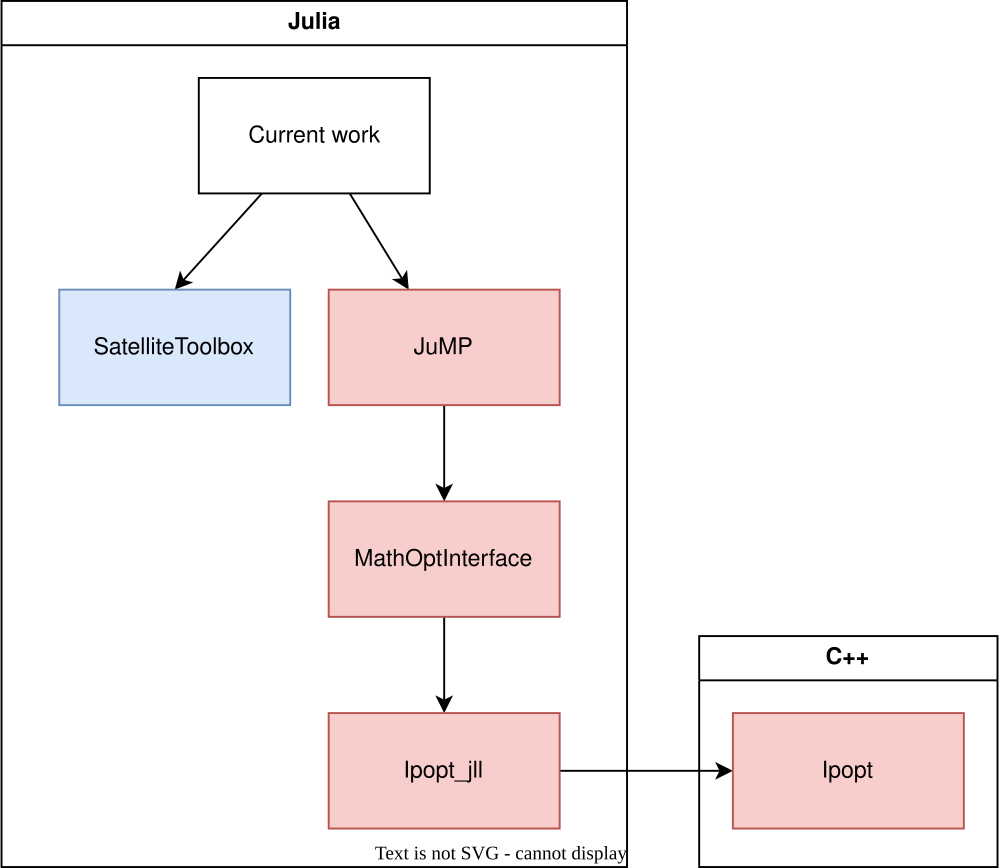
\includegraphics[width=\textwidth]{img/techstack.png}
    \caption{Relationship of code components}
    \label{fig:tech_stack}
\end{figure}

\section{Lambert problem implementation}

The formulations stated in the previous chapter make for one-dimensional nonlinear programs, which leads to high performance. However, they do not handle the singularity case of \(r_1 \parallel r_2\), which is of particular importance to orbital maneuvers as they often happen at periapsis and apoapsis. Sukhanov's formulation actually gives expressions for the initial radial and normal velocity when the input positions are collinear; the plane of the orbit should then be adequately chosen afterwards. However, this was found to be very numerically sensitive and another algorithm was used in the rest of this work. An implicit orbit propagation algorithm, as described in Section~\ref{sec:orbit_propagation} is setup with boundary conditions

\begin{align}
    r_{(j=1)} &= r_1 \\
    r_{(j=N+1)} &= r_2
\end{align}
which account for the 6 boundary conditions needed. In order to help convergence in the collinear case (and neighboring cases), two inequality constraints may be added:
\begin{align}
    r_j^T r_j &\geq R_{\text{Earth}}^2 \\
    r_j \times v_j &\geq 0
\end{align}
where the second constraint must be inverted if the desired orbit is retrograde. 

The propagation variables are initialized with the initial position and velocity.

\section{Optimal impulsive maneuver problem statement}\label{sec:impulsive_statement}

The full optimization problem, as it is implemented in code, shall be stated in this section. Due to \texttt{JuMP}'s intuitive modelling language, the problem is coded almost as it is stated here. The input parameters are:
\begin{enumerate}
    \item \(r_1\), \(v_1\): initial orbital position and velocity;
    \item \(r_2\), \(v_2\): final orbital position and velocity;
    \item \(t_f\): transfer time;
    \item \(N\): number of integration steps per coasting arc.
\end{enumerate}

The problem comprises the following variables, where inequalities represent variable bounds:
\begin{enumerate}
    \item \(\Delta t_1 \geq 0\), \(\Delta t_2 \geq 0\): intervals between 0 and the first maneuver and between the first and second maneuver;
    \item \(\Delta v_1 \geq 0\), \(\Delta v_2 \geq 0\)\footnote{The problem could have been parameterized with vector quantities for the changes in velocities, \(\Delta \vec v\), but the objective function would then be stated \(\sum \sqrt{\Delta \vec v^T \Delta \vec v}\), which is not differentiable at \(\Delta \vec v = 0\), which is inconvenient.}: magnitudes of the first and second impulses;
    \item \(\hat u 1\), \(\hat u_2 \in \mathbb{R}^3\): directions of the first and second impulses;
    \item \(\chi_1\), \(\chi_2\), \(\chi_3 \in \mathbb{R}^{6 \times (N+1)}\): arrays of state variables for each coasting arc. They shall be indexed as \(\chi_c^{kj}\), \(c=1, 2, 3\) is the coasting arc index, \(k=1,\dots,6\) is the component index, \(j = 1,\dots,N+1\) is the state vector index. \(X^j_c, r^j_c, v^j_c\) denote the j-th state , position and velocity vectors of the c-th coasting arc: \((X^j_c)_k = \chi_c^{kj}\).
\end{enumerate}

These variables are then subjected to constraints:
\begin{align}
    \text{Total time less than transfer time} &\qquad\Delta t_1 + \Delta t_2 \leq t_f \\
    \text{Unit directions} &\qquad\Delta \hat{u}_m^T \Delta \hat{u}_m = 1, m = 1, 2 \\
    \text{Initial state} &\qquad \chi_1^{k, 1} = \begin{bmatrix}
        r_1 \\ v_1
    \end{bmatrix}_k, k = 1,\dots, 6 \\
    \text{Final state} &\qquad \chi_3^{k, N+1} = \begin{bmatrix}
        r_2 \\ v_2
    \end{bmatrix}_k, k = 1,\dots, 6 \\
    \text{Maneuver boundary conditions} &\qquad \chi_{m+1}^{k, 1} = \chi_m^{k, N+1} + \begin{bmatrix}
        0_{3\times1} \\ \Delta v_m \hat{u}_m
    \end{bmatrix}, m=1, 2 \\
    \text{Propagation of coasting arcs} &\qquad X_c^{j+1} = f_{RK}(X_c^j, \Delta t_c / N), c=1, 2, 3, j=1,\dots,N \\
    \text{where} & \qquad \Delta t_3 = t_f - \Delta t_1 - \Delta t_2 \\
    % \text{Prograde orbit} &\qquad r^j_c \times v^j_c \geq 0, \forall j, c \\
    % \text{Non-intersection with Earth} &\qquad (r^j_c)^T r^j_c \geq R_{\text{Earth}}^2
\end{align}

Finally, the objective is given by
\begin{equation}
    \min \Delta v_1 + \Delta v_2
\end{equation}

The solver should be initialized with a feasible, but not necessarily optimal solution, for better convergence (since Ipopt is a local solver, the choice of initial guesses is important). Values for \(\Delta t_1\) and \(\Delta t_2\) should be proposed based on physical reasoning. Then, the variables of the first and last coasting arcs are initialized with direct orbital propagation results (computed with the \texttt{SatelliteToolbox} package). The second coasting arc, between the impulses, is initialized with the solution to the Lambert problem between the final position of the first coasting arc and the initial position of the last coasting arc. Finally, the variables concerning the impulses' magnitudes and directions are initialized with the difference in velocity between consecutive arcs.

\chapter{\textbf{Results}}

The theory and methods exposed previously are to be tested with concrete numerical examples, as well as be improved and expanded. In this chapter, an outline for expected results and deliverables of this work is given, as well as a simple numerical example: that of a Hohmann transfer in LEO. 

\section{Expected results}

Future deliverables shall include:
\begin{enumerate}
    \item A more robust code, capable of handling: 
    \begin{enumerate}
        \item multiple impulses;
        \item multiple revolution transfers;
        \item perturbed orbital dynamics;
    \end{enumerate}
    \item Estimation of feasible transfer times \(t_f\), which is currently treated as an arbitrary input;
    \item Analysis of more complex, practical orbital transfer cases under appropriate models (to be defined, but likely J2-perturbed dynamics):
    \begin{enumerate}
        \item LEO orbit maintenance: simultaneous correction in inclination and altitude;
        \item Sun synchronous orbit maintenance: correction in inclination, RAAN and semimajor-axis;
        \item Constellation phasing: coplanar maneuver to correct a satellite's phase (true anomaly) on a circular orbit;
        \item LEO to GEO transfer: multiple impulse, small plane change, numerical challenge (different time and spatial scales between the start and the end)
        \item \textbf{Optional}: plan series of impulses to use a Moon's gravity assist to increase scape velocity.
    \end{enumerate}
\end{enumerate}

\section{Preliminary results: Hohmann Transfer}

To validate the models created, a Hohmann transfer scenario is solved through direct optimization, and this solution is verified with primer vector theory and the known Hohmann transfer analytical solution.

The input orbital elements are given in table~\ref{tab:hohmann_orb_elems} and the orbits can be visualized in Figure~\ref{fig:hohmann_condition}. The blue dot is the initial position of the satellite and the yellow, its target position at the end of the control period. The lines represent the direction of the velocity.

\begin{table}[htbp]
    \centering
    \begin{tabular}{ccc} \toprule
        Element & Initial & Final \\ \midrule
        \(a\)      & \(7000\) km   & \(9000\) km   \\
        \(e\)      & \(0\)        & \(0\)        \\
        \(i\)      & \(51^\circ\) & \(51^\circ\) \\
        \(\Omega\) & \(0^\circ\)  & \(0^\circ\)  \\
        \(\omega\) & \(0^\circ\)  & \(0^\circ\)  \\
        \(\theta\) & \(0^\circ\)  & \(180^\circ\)  \\ \bottomrule
    \end{tabular}
    \caption{Orbital elements used for the Hohmann transfer case analysis}
    \label{tab:hohmann_orb_elems}
\end{table}

\begin{figure}[htbp]
    \centering
    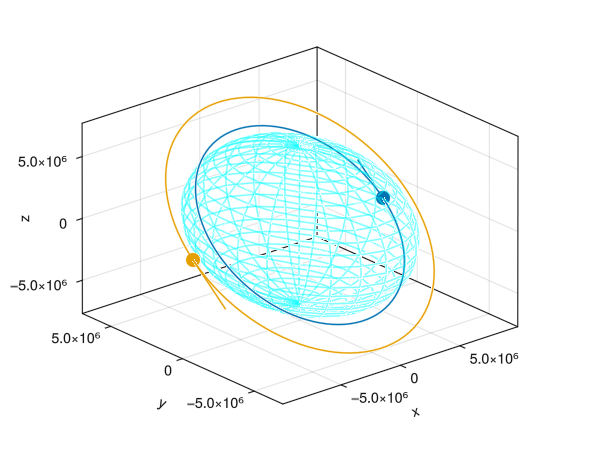
\includegraphics[width=0.6\textwidth]{img/hohmann_condition.png}
    \caption{Initial and final orbits for Hohmann transfer case visualization.}
    \label{fig:hohmann_condition}
\end{figure}

The total time was set to be equal to the analytical Hohmann transfer time\footnote{Methods for establishing how much time is needed for a certain maneuver shall be discussed in future results}, which from Equation~\eqref{eq:hohmann_time} is calculated as \(t_f = 3560.54\) s. Also from the analytical solution for the total change in velocity required, given in Equation~\eqref{eq:hohmann_deltav}, \(\sum \lVert \Delta v \rVert = 887.56\) m/s.

Initial guesses for \(\Delta t_1\) and \(\Delta t_2\) were arbitrarily proposed to be \(\frac{t_f}{3}\). The solution of the Lambert problem for the second coasting arc can be visualized in Figure~\ref{fig:hohmann_lambert}. Naturally, this solution is very far from optimal but it is feasible, which is what is expected of it.

\begin{figure}[htbp]
    \centering
    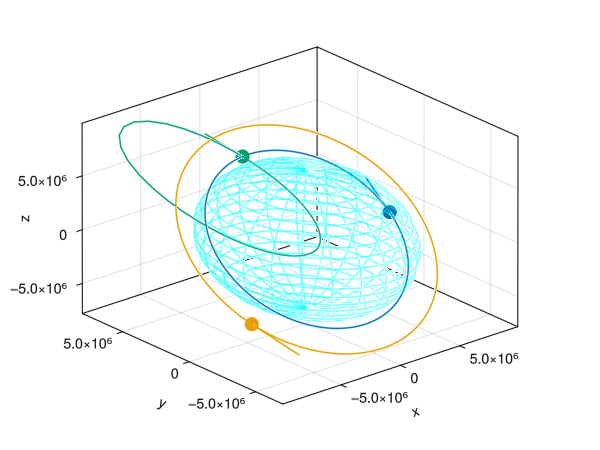
\includegraphics[width=0.6\textwidth]{img/hohmann_lambert_guess.png}
    \caption{Lambert problem solution for second coasting arc in Hohmann transfer case. This solution will serve as initial guess for the optimizer.}
    \label{fig:hohmann_lambert}
\end{figure}

Then, a discretization with \(N = 50\) was chosen. It was found that few steps lead to fast but imprecise solutions, which can often lead to infeasibility error conditions since the model is imprecise. Conversely, too many steps take much longer for no tangible gain in precision. The values of some variables are presented in table~\ref{tab:hohmann_results}, along with the expected analytical values. The solved, discretized trajectory can be seen in Figure~\ref{fig:hohmann_traj}.

\begin{table}[htbp]
    \centering
    \begin{tabular}{ccc} \toprule
        Variable & Analytical & Solver \\ \midrule
        \(\Delta t_1\) & 0s & 8e-4s \\
        \(\Delta t_2\) & 3560.54s & 3560.538s \\
        \(\sum \lVert \Delta v \rVert\) & \(887.56m/s\) & \(887.56m/s\) \\ \bottomrule
    \end{tabular}
    \caption{Comparison of optimized and analytical values of some important variables in the Hohmann transfer case.}
    \label{tab:hohmann_results}
\end{table}

\begin{figure}[htbp]
    \centering
    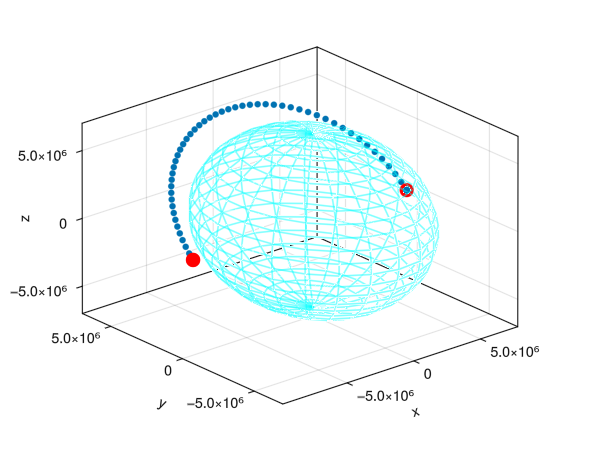
\includegraphics[width=0.6\textwidth]{img/hohmann_solved.png}
    \caption{Discretized transfer trajectory found by the numerical solver for the Hohmann transfer case.}
    \label{fig:hohmann_traj}
\end{figure}

Finally, primer vector theory is applied to verify is the found solution satisfies the optimality conditions. As a reminder, the number of impulses is not subjected to optimization and must be interactively changed based on primer vector trajectory results. The trajectory of the primer vector norm and its derivative are shown in Figure~\ref{fig:hohmann_primer_vec}. The trajectory of the norm is continuous, and always less than 1, except for the impulse instants, when it has norm exactly one. Thus, the necessary conditions are satisfied and no modifications to the optimized trajectory can be extracted from the primer vector history.

\begin{figure}[htbp]
    \centering
    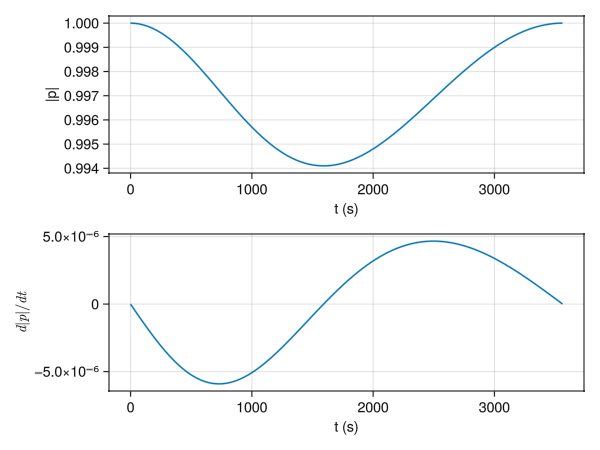
\includegraphics[width=0.6\textwidth]{img/hohmann_primer_vector_history.png}
    \caption{Primer vector norm and norm time-derivative trajectories for Hohmann transfer case.}
    \label{fig:hohmann_primer_vec}
\end{figure}

% \chapter{\textbf{Planning}}
% A Gantt chart for the planned work is presented in Figure~\ref{fig:planning}. The planning is optimistic and the most risky section is the improvement of the code, in particular the addition of multiple revolution transfers. Thus, plenty of time has been allocated to these tasks.

\begin{figure}[htbp]
    \centering
    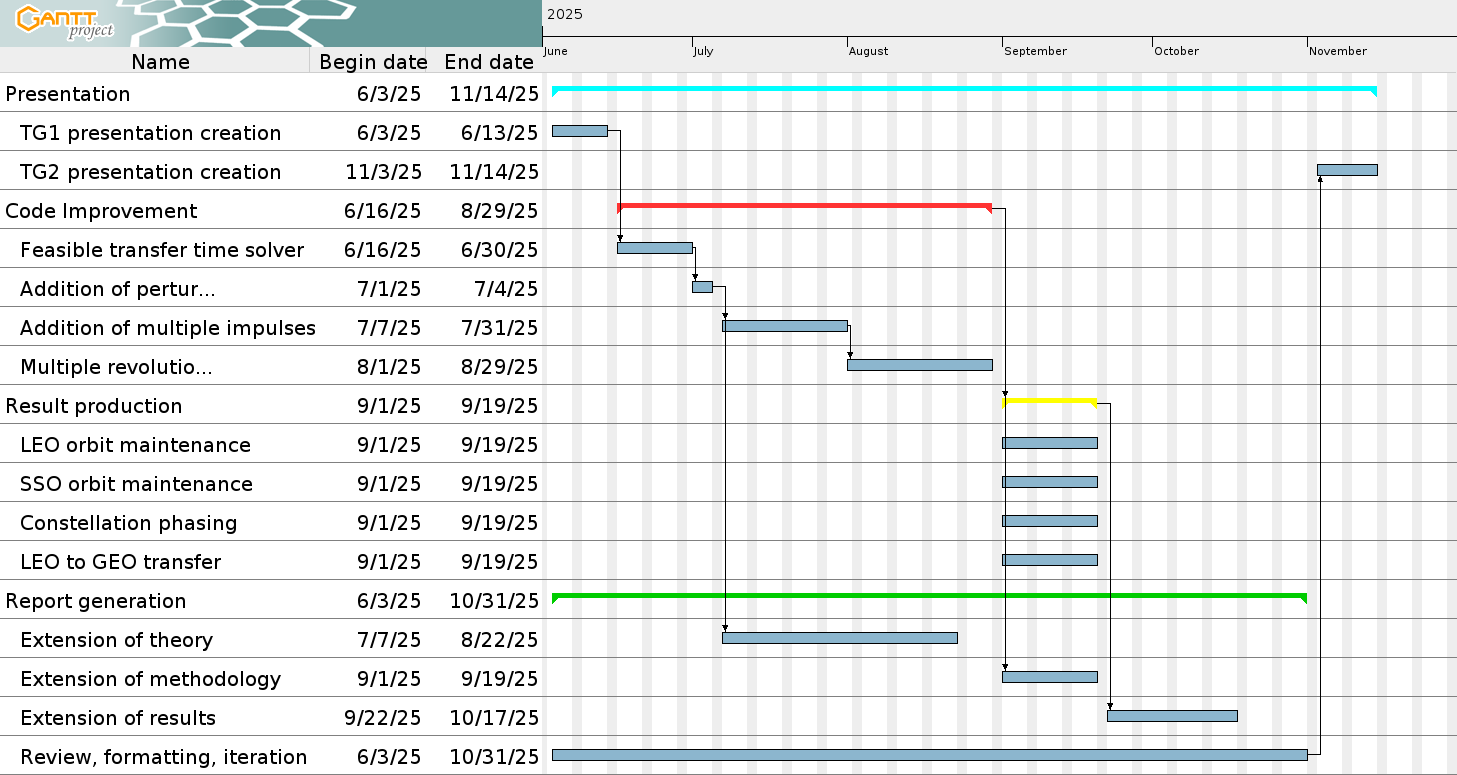
\includegraphics[width=\textwidth]{img/TG planning.png}
    \caption{Gantt Chart of planned workload.}
    \label{fig:planning}
\end{figure}
\chapter{Conclusion}
In summary, this work set out to apply primer vector theory to optimal impulse maneuvers in LEO and adapt it to the types of perturbations encountered in this environment. An impulsive multiple shooting optimization scheme in Cartesian coordinates was successfully implemented, and validated under Keplerian dynamics for the well known Hohmann transfer case, and for a more complex noncoplanar rendez-vous scenario proposed in the primer vector literature. The same scenarios were solved under conservative and non-conservative perturbation models, allowing for the comparison of the effect of perturbations in the optimal maneuvers and in the primer vector algorithm. For each model, some valid methods of primer vector calculation have been tried and validated between each other, and the primer vector has proven to be a useful tool in reducing the cost of orbital maneuvers. As for the perturbations, the modelling of the J2 force greatly alters the nature of orbital maneuvers, mainly due to the fact that orbits are no longer planar. The addition of drag in the orbital model does not alter significantly the optimal maneuvers or the primer vector analysis, which allows the usage of the STM method for its calculation, even though in general it is predicted that the STM method will not work for non-conservative models. 

Future works might investigate under which conditions the effects of drag alter orbital maneuvers and the primer vector trajectories, as well as increase the time horizon of the maneuvers considered. In addition, the exploration of possible performance gains from using modified equinoctial elements instead of a Cartesian formulation might be investigated. Lastly, no general method for estimating lower bounds of maneuver costs is known; the methods presented in this work would greatly profit from a lower bound estimation.

TODO checklist, 

TODO agradecimentos

TODO reler

TODOformatação
% REFERENCIAS BIBLIOGRAFICAS
\renewcommand\bibname{\itareferencesnamebabel} %renomear título do capítulo referências
\bibliography{Referencias/referencias}

% Apendices
\appendix
% \chapter{Future Planning}
\chapter{Generating random numbers with constant sum}\label{app:random_sum}

The goal is to generate a set of \(n\) numbers \((\x)_{1 \leq i \leq n} \in [0, 1]\) such that
\begin{equation}
    \sum_{i=1}^{n} \x_i = 1
\end{equation}
with uniform distribution on the set \(\Omega = \{\x \in [0, 1]^n \mid \sum_{i=1}^{n} \x_i = 1 \}\). The procedure relies on rejection sampling in \(n-1\) dimensions since the set \(\Omega\) has probability 0 in the space \([0, 1]^n\). Generate a random sample \(\mathbf{z} \in [0, 1]^{n-1}\) and reject it if
\begin{equation}
    \sum_{i=1}^{n-1} \mathbf{z}_i > 1.
\end{equation}

Otherwise, accept the sample and set
\begin{align}
    \x_i &= \mathbf{z}_i, i = 1,\dots,n-1 \\
    \x_n &= 1 - \sum_{i=1}^{n-1} \x_i.
\end{align}

% Anexos
\annex

% Glossario
%\itaglossary
%\printglossary

% Folha de Registro do Documento
% Valores dos campos do formulario
\FRDitadata{25 de março de 2015}
\FRDitadocnro{DCTA/ITA/DM-018/2015} %(o número de registro você solicita a biblioteca)
\FRDitaorgaointerno{Instituto Tecnológico de Aeronáutica -- ITA}
%Exemplo no caso de pós-graduação: Instituto Tecnol{\'o}gico de Aeron{\'a}utica -- ITA
\FRDitapalavrasautor{Cupim; Cimento; Estruturas}
\FRDitapalavrasresult{Propulsão; Gás Frio; Vetorização de empuxo;}
%Exemplo no caso de graduação (TG):
%\FRDitapalavraapresentacao{Trabalho de Graduação, ITA, São José dos Campos, 2015. \NumPenultimaPagina\ páginas.}
%Exemplo no caso de pós-graduação (msc, dsc):
\FRDitapalavraapresentacao{ITA, São José dos Campos. Curso de Mestrado. Programa de Pós-Graduação em Engenharia Aeronáutica e Mecânica. Área de Sistemas Aeroespaciais e Mecatrônica. Orientador: Prof.~Dr. Adalberto Santos Dupont. Coorientadora: Prof$^\textnormal{a}$.~Dr$^\textnormal{a}$. Doralice Serra. Defesa em 05/03/2015. Publicada em 25/03/2015.}
\FRDitaresumo{Este trabalho apresenta o processo de desenvolvimento e caracterização de um sistema de vetorização de empuxo com motor a gás frio. O motor tem como requisito empuxo de \(2\;\mathrm{N}\) e \(5\;\mathrm{bar}\) de pressão de câmara. O método de vetorização escolhido para teste foi o de \textit{jet vane}. O motor construído apresentou divergências pequenas com os requisitos, tendo um impulso específico de \(46,6\;\mathrm{s}\). Este motor foi montado em um mecanismo de controle da lâmina defletora e esta montagem foi acoplada a uma balança de três componentes para caracterização das forças e momentos gerados. Como resultado final, obtiveram-se as derivadas de controle de força lateral e momento. Por fim, apresentaram-se os problemas metodológicos encontrados e \textit{trade-offs} de engenharia identificados para o sistema.}
%  Primeiro Parametro: Nacional ou Internacional -- N/I
%  Segundo parametro: Ostensivo, Reservado, Confidencial ou Secreto -- O/R/C/S
\FRDitaOpcoes{N}{O}
% Cria o formulario
\itaFRD

\end{document}
% Fim do Documento. O massacre acabou!!! :-)
